\documentclass{article}


% if you need to pass options to natbib, use, e.g.:
%     \PassOptionsToPackage{numbers, compress}{natbib}
% before loading neurips_2023


% ready for submission
% \usepackage{neurips_2023}


% to compile a preprint version, e.g., for submission to arXiv, add add the
% [preprint] option:
  \usepackage[preprint]{neurips_2023}


% to compile a camera-ready version, add the [final] option, e.g.:
  % \usepackage[final]{neurips_2023}


% to avoid loading the natbib package, add option nonatbib:
  %  \usepackage[nonatbib]{neurips_2023}


\usepackage[utf8]{inputenc} % allow utf-8 input
\usepackage[T1]{fontenc}    % use 8-bit T1 fonts
\usepackage{hyperref}       % hyperlinks
\usepackage{url}            % simple URL typesetting
\usepackage{booktabs}       % professional-quality tables
\usepackage{amsfonts}       % blackboard math symbols
\usepackage{nicefrac}       % compact symbols for 1/2, etc.
\usepackage{microtype}      % microtypography
\usepackage{xcolor}         % colors
\usepackage{graphicx}       % Required for including graphics
\usepackage{subcaption}     % Required for subfigure environment
\usepackage{listings}       % Required for lstlisting environment
\usepackage{float}          % Enables tables to be rendered anywhere on the page
\usepackage{amsmath}        % For math environments like equation
\usepackage{pgfplots}       % For histogram
\usepackage{tikz}           % For histogram
\pgfplotsset{compat=1.18}


\title{BME1312 Project1 Report: Deep Learning for MRI Reconstruction}


% The \author macro works with any number of authors. There are two commands
% used to separate the names and addresses of multiple authors: \And and \AND.
%
% Using \And between authors leaves it to LaTeX to determine where to break the
% lines. Using \AND forces a line break at that point. So, if LaTeX puts 3 of 4
% authors names on the first line, and the last on the second line, try using
% \AND instead of \And before the third author name.


\author{%
  Wenye Xiong \\
  2023533141 \\
  \texttt{xiongwy2023@shanghaitech.edu.cn}
  \And
  Renyi Yang \\
  2023533030 \\
  \texttt{yangry2023@shanghaitech.edu.cn}
  \AND
  Jiaxing Wu \\
  2023533160 \\
  \texttt{wujx2023@shanghaitech.edu.cn}
  \And
  Boyang Xia \\
  2023533073 \\
  \texttt{xiaby2023@shanghaitech.edu.cn}
  \AND
  Fengmin Yang \\
  2023533183 \\
  \texttt{yangfm2023@shanghaitech.edu.cn}
}

\begin{document}


\maketitle


\begin{abstract}
  This project uses deep learning to reconstruct high-quality dynamic MRI images
  from undersampled data. We propose a deep-learning-based denoising framework combining
  two independent UNet modules (processing real and imaginary components separately) and a 3D ResNet to explore the temporal correlation.
  We generate variable density undersampling patterns with acceleration factor 5 and
  11 central k-space lines per frame, analyze the resulting aliasing artifacts, and evaluate
  reconstruction performance with PSNR and SSIM metrics. Additionally,
  we investigate the effects of dropout, dynamic learning rate schedules,
  and compare L1 versus L2 losses. Finally, we explore an unrolled network architecture
  incorporating data consistency layers between cascaded instances of our base reconstruction network.
  Access our code, dataset, and results at \url{https://github.com/XiongWenye/Deep-Learning-Dynamic-MRI-Reconstruction}.
\end{abstract}

\section{Introduction}
Dynamic magnetic resonance imaging (MRI) enables visualization of physiological processes by capturing multiple images over time, but faces a fundamental tradeoff between spatial resolution, temporal resolution, and scan duration. Accelerated MRI acquisition through k-space undersampling can address this challenge but introduces aliasing artifacts that degrade image quality. This project explores deep learning approaches to reconstruct high-quality dynamic MRI images from significantly undersampled k-space data (acceleration factor 5).

We develop and evaluate a novel reconstruction framework with three key components: (1) a dual-branch UNet architecture to separately process real and imaginary components of complex MRI data, (2) a 3D ResNet to leverage temporal correlations across dynamic frames, and (3) data consistency layers in an unrolled network configuration to enforce fidelity to the acquired measurements. Throughout our experiments, we investigate how different design choices—including dropout regularization, learning rate schedules, loss functions, and network architecture—affect reconstruction quality as measured by Peak Signal-to-Noise Ratio (PSNR) and Structural Similarity Index (SSIM).

This report documents our methodology, implementation details, experimental results, and analysis across five main sections: undersampling pattern generation, network architecture design, ablation studies on regularization techniques, comparison of loss functions, and exploration of unrolled network architectures. Our findings provide practical insights for designing effective deep learning solutions for dynamic MRI reconstruction.


\section{Variable Density Random Undersampling Pattern Generation and Aliasing Artifacts Analysis}
\textit{Note: }You may need \texttt{train.py}, line 29, function \texttt{variable\_density\_mask()}
and line 456, function \texttt{process\_data()} for reference in this section.

\subsection{Undersampling Pattern Generation}
We were asked to generate a variable density random undersampling mask $U$ matching the cine
dataset size, with acceleration factor 5 and 11 fully sampled central k-space lines per frame.
The mask values are 1 at sampled locations and 0 otherwise.

The provided code generates a 4D undersampling mask (shape [batch, frames, height, width]) using the following steps:
\begin{enumerate}
  \item Initialization: A zero-initialized mask is created with the input shape.
  \item Central Region Sampling: For each frame, 11 central k-space lines are
        sampled to retain low-frequency spatial information.
  \item Variable Density Probability Distribution: A quadratic probability density
        function is defined, decreasing with distance from the k-space center.
  \item Random Peripheral Sampling: The remaining lines are sampled randomly
        based on the probability distribution we obtained.
  \item Dynamic Frame Variability: Each dynamic frame independently generates
        unique random peripheral lines to ensure temporal incoherence of aliasing artifacts.
\end{enumerate}

\subsection{Undersampling Masks Plotting}
Figure \ref{fig:undersampling_mask} shows the undersampling mask for one dynamic frame and undersampling masks in the ky-t dimension.

\begin{figure}[H]
  \centering
  \includegraphics[width=\linewidth]{../assets/undersampling_mask.png}
  \caption{Undersampling Mask for one dynamic frame and undersampling masks in the ky-t dimension.}
  \label{fig:undersampling_mask}
\end{figure}

Thus we can see that the sampling mask is not the same for different dynamic frames.
That's because sampling positions are randomized per frame to disrupt coherent aliasing artifacts in time. Figure \ref{fig:multiple_masks} shows masks for multiple frames.

\begin{figure}[H]
  \centering
  \includegraphics[width=0.8\linewidth]{../assets/mask.png}
  \caption{Multiple sampling masks showing the variable density patterns across different temporal frames.}
  \label{fig:multiple_masks}
\end{figure}

\subsection{Aliased Images Depiction and Comparison}
From the stem of this question we can know that, given a fully sampled image $m$,
the aliased image $b$ is computed as: 
\begin{center}
  $b = F^{-1} U F m$
\end{center}
where $F$ is the Fourier transform.

In function \texttt{process\_data()}, we first load the dynamic MRI dataset dataset from the \texttt{cine.npz} file,
and convert the data into PyTorch tensor labels, which are used as ground truth for subsequent processing. Then we
call the function \texttt{variable\_density\_mask()} that we've just implemented to generate a mask,
and then apply the mask to the k-space data, and convert the fully sampled image data to the frequency
domain by Fourier transform (\texttt{image2kspace}). After that, we undersample the k-space data through the mask,
and perform an inverse Fourier transform (\texttt{kspace2image}) on the undersampled k-space to generate an aliased image.

Figure \ref{fig:comparison_images} compares the fully sampled image, aliased image, and sampling mask in Fourier domain.
Here we choose the first 3 images generated to better compare the aliased images with the fully sampled image.

\begin{figure}[H]
  \centering
  \begin{subfigure}[b]{\linewidth}
    \includegraphics[width=\linewidth]{../assets/comparison_image_0.png}
    \caption{Comparison for frame 0}
    \label{fig:comparison_image_0}
  \end{subfigure}
  \quad
  \begin{subfigure}[b]{\linewidth}
    \includegraphics[width=\linewidth]{../assets/comparison_image_1.png}
    \caption{Comparison for frame 1}
    \label{fig:comparison_image_1}
  \end{subfigure}
  \quad
  \begin{subfigure}[b]{\linewidth}
    \includegraphics[width=\linewidth]{../assets/comparison_image_2.png}
    \caption{Comparison for frame 2}
    \label{fig:comparison_image_2}
  \end{subfigure}
  \caption{Comparison between fully sampled (left), undersampled (middle), and corresponding sampling mask (right) for different frames.}
  \label{fig:comparison_images}
\end{figure}

Description of aliased images: Since the low-frequency information in the center k-space
is usually better preserved, the main structure of the image is displayed more clearly;
however, due to the lack of high-frequency information, the edges of the image are
blurred with repetitive ripples (i.e., artifacts), especially in dynamic imaging,
where the artifacts vary with time frames.

Comparison of aliasing image and fully sampled image: fully sampled image retains
complete high-frequency information, with clear and detailed edges and no artifacts,
whereas aliasing image has reduced resolution due to insufficient high-frequency
sampling and produces artifacts.


\newpage
\section{Dataset Partition, Denoising Network Construction and Evaluation}
\textit{Note: }You may need \texttt{train.py}, line 113, class \texttt{UNet};
line 345, class \texttt{ResNet} and line 497, function \texttt{train()}
for reference in this section. (Some related functions are also needed)
\subsection{Dataset Partition}
The full dataset contains 200 samples is split into training, validation, and testing sets with ratios 4:1:2, resulting in 114 training, 29 validation,
and 57 testing samples.
\subsection{CNN Network Designing and Training}
Our reconstruction network consists of three components:
\begin{enumerate}
   \item \textbf{Dual 2D UNet Architecture:} Two independent UNet modules process the real and imaginary parts of the complex MRI data separately. Each UNet features an encoder-decoder structure with skip connections. A key component is our implementation of dual attention mechanisms: channel attention that recalibrates feature maps by explicitly modeling interdependencies between channels, and spatial attention that focuses on informative regions by selectively emphasizing important spatial locations. These attention modules significantly enhance feature representation by suppressing irrelevant features and highlighting diagnostically important structures. The UNet architecture also incorporates dropout (p=0.3) for regularization and LeakyReLU activation for improved gradient flow during training.
    \item \textbf{Concatenation:} The outputs of the two UNet branches are concatenated along the channel dimension, preserving the complementary spatial information extracted from both real and imaginary components.
    \item \textbf{3D ResNet (Temporal Fusion):} While the UNet branches effectively extract spatial features, temporal correlation between consecutive frames remains unexploited. To address this, we employ a lightweight 3D ResNet that processes the concatenated features through 3D convolutions and residual connections. This temporal fusion module captures dynamic changes across the MRI sequence, leveraging both short-term and long-term dependencies between adjacent frames. By incorporating both spatial context (from UNets) and temporal dynamics (from ResNet), our model effectively suppresses time-varying artifacts and produces temporally coherent reconstructions. A final 1x1x1 convolution maps the spatio-temporal features to the output channels.
\end{enumerate}
This design (shown in Figure \ref{fig:pipeline}) effectively utilizes both spatial information (2D UNet processing) and temporal information (capturing dynamic changes via 3D ResNet) for the reconstruction task.
\begin{figure}[H]
  \centering
  \includegraphics[width=0.85\linewidth]{../assets/pipeline.png}
  \caption{Overall architecture of our proposed reconstruction network with dual UNet branches for real and imaginary components and 3D ResNet for temporal fusion.}
  \label{fig:pipeline}
\end{figure}

We first train a baseline network \textbf{without} dropout and dynamic learning rate schedule, using a constant learning rate. The parameters are: Adam optimizer, initial learning rate $10^{-4}$, weight decay $10^{-4}$, batch size 10, and $L2$ loss (MSE). Training and validation losses are logged per epoch.

All the training loss and validation loss are recorded in the file named \texttt{output/No\_opt\_output.txt}.
The loss curves for 800 epochs are plotted in Figure \ref{fig:loss_no_opt}.
\begin{figure}[H]
  \centering
  \includegraphics[width=0.7\linewidth]{../assets/Training Loss and Validation Loss No opt.png}
  \caption{Training Loss and Validation Loss (No Dropout/Dynamic LR)}
  \label{fig:loss_no_opt}
\end{figure}

In Figures \ref{fig:full_sampled_no_opt}-\ref{fig:reconstructed_no_opt}, we show example testing images before and after deep learning reconstruction using this baseline model. The complete results can be found in the folder \texttt{images/No\_opt}.

\begin{figure}[H]
  \centering
  \begin{subfigure}[b]{0.32\linewidth}
    \includegraphics[width=\linewidth]{../images/No_opt/full_sampling/full_sampling_0.png}
    \caption{Frame 0}
  \end{subfigure}
  \begin{subfigure}[b]{0.32\linewidth}
    \includegraphics[width=\linewidth]{../images/No_opt/full_sampling/full_sampling_1.png}
    \caption{Frame 1}
  \end{subfigure}
  \begin{subfigure}[b]{0.32\linewidth}
    \includegraphics[width=\linewidth]{../images/No_opt/full_sampling/full_sampling_2.png}
    \caption{Frame 2}
  \end{subfigure}
  \caption{Fully Sampled Images (Ground Truth)}
  \label{fig:full_sampled_no_opt}
\end{figure}

\begin{figure}[H]
  \centering
  \begin{subfigure}[b]{0.32\linewidth}
    \includegraphics[width=\linewidth]{../images/No_opt/under_sampling/under_sampling_0.png}
    \caption{Frame 0}
  \end{subfigure}
  \begin{subfigure}[b]{0.32\linewidth}
    \includegraphics[width=\linewidth]{../images/No_opt/under_sampling/under_sampling_1.png}
    \caption{Frame 1}
  \end{subfigure}
  \begin{subfigure}[b]{0.32\linewidth}
    \includegraphics[width=\linewidth]{../images/No_opt/under_sampling/under_sampling_2.png}
    \caption{Frame 2}
  \end{subfigure}
  \caption{Under Sampled Images (Input to Network)}
  \label{fig:under_sampled_no_opt}
\end{figure}

\begin{figure}[H]
  \centering
  \begin{subfigure}[b]{0.32\linewidth}
    \includegraphics[width=\linewidth]{../images/No_opt/reconstruction/reconstruction_0.png}
    \caption{Frame 0}
  \end{subfigure}
  \begin{subfigure}[b]{0.32\linewidth}
    \includegraphics[width=\linewidth]{../images/No_opt/reconstruction/reconstruction_1.png}
    \caption{Frame 1}
  \end{subfigure}
  \begin{subfigure}[b]{0.32\linewidth}
    \includegraphics[width=\linewidth]{../images/No_opt/reconstruction/reconstruction_2.png}
    \caption{Frame 2}
  \end{subfigure}
  \caption{Reconstruction Images (Baseline Model - No Dropout/Dynamic LR)}
  \label{fig:reconstructed_no_opt}
\end{figure}

Comment on the denoising/dealiasing performance (Baseline Model):
\begin{enumerate}
  \item Denoising: The network reduces some noise compared to the undersampled input, but residual noise and artifacts remain.
  \item Dealiasing: The network attempts to reduce aliasing artifacts, but the reconstruction quality is limited, and some blurring and artifact patterns persist.
\end{enumerate}

\subsection{Quantitative Evaluation (Baseline Model)}
After calculating the PSNR and SSIM for each testing slice before and after deep learning reconstruction using the baseline model (no dropout/dynamic LR), we get:
\begin{enumerate}
  \item The mean of PSNR: 24.15409541, the standard deviation of PSNR: 1.85842901
  \item The mean of SSIM: 0.74309104, the standard deviation of SSIM: 0.03733812
\end{enumerate}
These metrics indicate moderate reconstruction quality. The validation loss curve (Figure \ref{fig:loss_no_opt}) shows fluctuations and a potential increase towards the end, suggesting overfitting, which limits performance.



\section{Impact of Dropout and Dynamic Learning Rate}
\textit{Note: }Detailed reconstruction images, related training loss, validation loss and their
loss curves for the optimized model can be found in \texttt{assets/Training Loss and Validation Loss.png},
\texttt{output/output.txt} and \texttt{images/output}.\\
We now train our full model, incorporating dropout (p=0.3 in UNet) and a cosine annealing learning rate schedule with warm-up. The code can be found in \texttt{class UNet} and \texttt{function train()}. The training parameters are otherwise the same (Adam, initial LR $10^{-4}$, weight decay $10^{-4}$, batch size 10, L2 loss, 800 epochs).

By calculating the PSNR and SSIM again for this optimized model, we can compare it with the baseline (Table \ref{tab:opt_compare}).
\begin{table}[H]
  \caption{Compare PSNR and SSIM with and without Dropout/Dynamic LR}
  \label{tab:opt_compare}
  \centering
  \begin{tabular}{lllll}
    \toprule
    Optimization?    & PSNR mean   & PSNR std dev & SSIM mean  & SSIM std dev \\
    \midrule
    Before Recon    & 23.463965 & 2.866855 & 0.572510233579521 & 0.088547643071673 \\
    No               & 24.15409541 & 1.85842901   & 0.74309104 & 0.03733812   \\
    Yes (Full Model) & 29.08446121 & 1.93235576   & 0.84434632 & 0.03711063   \\
    \bottomrule
  \end{tabular}
\end{table}

Compared to the baseline, adding dropout and a dynamic learning rate significantly improves both PSNR and SSIM.
\begin{itemize}
  \item The mean PSNR increases from 24.15 to 29.08, indicating a substantial reduction in noise and error, making the reconstructed image much closer to the ground truth.
  \item The mean SSIM increases from 0.743 to 0.844, indicating a significant improvement in structural similarity. The model better captures the real structure of the image.
  \item The standard deviations remain relatively low and similar, suggesting consistent performance across the test set for both models, but the optimized model achieves this consistency at a much higher quality level.
\end{itemize}
These enhancements are due to:
\begin{enumerate}
  \item Dropout acts as a regularizer, reducing overfitting by preventing the network from relying too heavily on specific neurons or features in the training data. This improves generalization to unseen data and makes the model more robust to undersampling artifacts.
  \item The dynamic learning rate schedule (cosine annealing with warm-up) helps the training process. The warm-up phase stabilizes initial training, the cosine decay allows for faster convergence initially and then fine-tuning with smaller steps later, helping the model find a better minimum and improve detail recovery.
\end{enumerate}
The loss curves for the optimized model (Figure \ref{fig:loss_opt}) show much more stable convergence compared to the baseline (Figure \ref{fig:loss_no_opt}).

\begin{figure}[H]
  \centering
  \includegraphics[width=\linewidth]{../assets/Training Loss and Validation Loss.png}
  \caption{Training Loss and Validation Loss (Optimized Model with Dropout/Dynamic LR, L2 Loss)}
  \label{fig:loss_opt}
\end{figure}

\begin{figure}[H]
  \centering
  \includegraphics[width=0.8\linewidth]{../images/compare.PNG}
  \caption{Comparison of the reconstruction(left) and the ground truth(right) for frame 0.}
  \label{fig:compare}
\end{figure}

\section{Compare L1 with L2 Loss}
\textit{Note: }Detailed reconstruction images, related training loss, validation loss and their
loss curves can be found in \texttt{assets/Training Loss and Validation Loss L1.png},
\texttt{output/L1\_Loss\_output.txt} and \texttt{images/L1}.\\
We replace the L2 loss (MSE) with L1 loss (MAE) in the training pipeline, retraining using the same optimized architecture (dropout, dynamic LR) and training parameters. We then compare the new PSNR and SSIM with the results from the optimized L2 model (Table \ref{tab:loss_compare}).

\begin{table}[H]
  \caption{Compare PSNR and SSIM with L1 vs L2 Loss (Optimized Model)}
  \label{tab:loss_compare}
  \centering
  \begin{tabular}{lllll}
    \toprule
    Loss & PSNR mean   & PSNR std dev & SSIM mean  & SSIM std dev \\
    \midrule
    Before Recon    & 23.463965 & 2.866855 & 0.572510233579521 & 0.088547643071673 \\
    L1   & 29.15108941 & 2.24063664   & 0.84389277 & 0.04208510   \\
    L2   & 29.08446121 & 1.93235576   & 0.84434632 & 0.03711063   \\
    \bottomrule
  \end{tabular}
\end{table}

We can see that L1 loss yields slightly higher mean PSNR, while L2 loss yields slightly higher mean SSIM and lower standard deviations for both metrics in the testing dataset.

This phenomenon can be explained as follows:
\begin{itemize}
  \item PSNR (Peak Signal-to-Noise Ratio) measures pixel-wise accuracy. L1 loss, by minimizing the mean absolute error, effectively reduces pixel-level discrepancies, thus improving PSNR.
  \item SSIM (Structural Similarity Index) evaluates structural similarity, focusing on local patterns of luminance, contrast, and structure. L1 loss does not explicitly enforce structural consistency. Small spatial misalignments or distortions, which might minimally impact PSNR, can significantly lower SSIM.
\end{itemize}
In short, L1 loss favors pixel-wise precision but may compromise local structural integrity. A potential solution could be a composite loss function combining L1 with a structure-aware loss like SSIM loss or a perceptual loss.

The training curve for L1 loss (Figure \ref{fig:loss_l1}) appears stable. While L1 loss can sometimes promote sparsity, L2 loss often leads to smoother results and is more sensitive to large errors. In this case, both loss functions yield comparable high-quality reconstructions. However, the original configuration with L2 loss achieved slightly better stability (lower standard deviation in metrics) and lower final validation loss values.

Ultimately, the choice of loss function should be guided by the final objective:
\begin{itemize}
  \item If precise pixel recovery is the goal, prioritizing PSNR with L1 or L2 loss may suffice.
  \item If maintaining perceptual quality and structural fidelity is crucial (e.g., in clinical imaging), incorporating structure-aware losses is strongly recommended.
\end{itemize}

\begin{figure}[H]
  \centering
  \includegraphics[width=\linewidth]{../assets/Training Loss and Validation Loss L1.png}
  \caption{Training Loss and Validation Loss (Optimized Model with L1 Loss)}
  \label{fig:loss_l1}
\end{figure}


\subsection{Application of Perceptual Loss and Edge Loss in MRI Reconstruction}

In MRI reconstruction tasks, especially under highly undersampled conditions, achieving both high numerical accuracy and perceptually pleasing images is crucial. Traditional pixel-wise losses such as Mean Squared Error (MSE) tend to produce blurry reconstructions, as they overly penalize small pixel mismatches without considering the structural or perceptual quality of the image.

\textbf{Perceptual loss} addresses this limitation by measuring the difference between the reconstructed and ground truth images in the feature space of a pre-trained convolutional neural network. This encourages the model to preserve high-level semantic features and fine textures.

\textbf{Edge loss}, on the other hand, focuses explicitly on preserving sharp structural details. By applying an edge detection operator (such as Sobel filters) to both the reconstructed and ground truth images and minimizing the difference between their edge maps, the network is guided to accurately recover critical high-frequency components, such as organ boundaries and anatomical structures, which are vital in medical imaging.

Combining perceptual loss and edge loss with traditional pixel-wise losses leads to reconstructions that are not only numerically superior but also visually much sharper and structurally more faithful to the original anatomy.

Due to the restrictions of the current project, we did not implement perceptual loss and edge loss in our training pipeline. We recommend exploring these advanced loss functions in future work to further enhance the quality of MRI reconstructions, especially in challenging undersampling scenarios.

\section{Creativity: Comparison with Attention Mechanisms}

To evaluate the impact of attention mechanisms, we incorporated channel attention and spatial attention modules into the baseline network. These modules were added to the encoder-decoder structure of the UNet branches to enhance feature representation by focusing on the most informative regions and channels.

The performance metrics for the attention-based model are compared with the baseline (optimized with dropout and dynamic LR) in Table \ref{tab:attention_compare}.

\begin{table}[H]
  \caption{Comparison of Baseline and Attention-Based Models}
  \label{tab:attention_compare}
  \centering
  \begin{tabular}{lllll}
    \toprule
    Model               & PSNR mean   & PSNR std dev & SSIM mean  & SSIM std dev \\
    \midrule
    Baseline (Optimized) & 29.08446121 & 1.93235576   & 0.84434632 & 0.03711063   \\
    Attention-Based      & 32.38721751 & 1.87722389   & 0.89100512 & 0.03601302   \\
    \bottomrule
  \end{tabular}
\end{table}

\subsection{Discussion}
\begin{itemize}
  \item \textbf{PSNR Improvement:} The attention-based model achieved a higher mean PSNR compared to the baseline, indicating better pixel-wise reconstruction accuracy.
  \item \textbf{SSIM Improvement:} The mean SSIM also improved, suggesting that the attention mechanisms helped preserve structural details more effectively.
  \item \textbf{Stability:} The standard deviations for both PSNR and SSIM were slightly lower in the attention-based model, indicating more consistent performance across the test set.
\end{itemize}

\subsection{Loss Curves}
The training and validation loss curves for the attention-based model are shown in Figure \ref{fig:loss_attention}. The curves demonstrate stable convergence, with lower final validation loss compared to the baseline.

\begin{figure}[H]
  \centering
  \includegraphics[width=\linewidth]{../assets/Training Loss and Validation Loss with attention.png}
  \caption{Training Loss and Validation Loss (Attention-Based Model)}
  \label{fig:loss_attention}
\end{figure}

\subsection{Visual Comparison}
Figure \ref{fig:attention_comparison} compares the reconstruction results of the attention-based models with full sampled one for a sample frame. 

\begin{figure}[H]
  \centering
  \begin{subfigure}[b]{0.32\linewidth}
    \includegraphics[width=\linewidth]{../images/with_attention/full_sampling/full_sampling_0.png}
    \caption{Ground Truth}
  \end{subfigure}
  \begin{subfigure}[b]{0.32\linewidth}
    \includegraphics[width=\linewidth]{../images/with_attention/reconstruction/reconstruction_0.png}
    \caption{Attention-Based Reconstruction}
  \end{subfigure}
  \caption{Comparison of Reconstruction Results (Frame 0)}
  \label{fig:attention_comparison}
\end{figure}

\subsection{Conclusion}
Incorporating attention mechanisms significantly improved both quantitative metrics (PSNR and SSIM) and visual quality. The attention modules enhanced the network's ability to focus on critical features, leading to sharper and more accurate reconstructions. Future work could explore combining attention mechanisms with unrolled architectures for further improvements.

\section{Unrolled Deep Learning Reconstruction Network}
We explored an unrolled network architecture incorporating data consistency (DC) layers between cascaded instances of our base reconstruction network (Dual UNet + 3D ResNet). The DC layer enforces consistency with the acquired k-space data after each denoising step using the formula:
$k_{out} = U \odot k_{undersampled} + (1 - U) \odot F(x_{denoised})$, where $k_{undersampled}$ is the initially acquired undersampled k-space data, $x_{denoised}$ is the output of the denoising network, $F$ is the Fourier transform, and $U$ is the undersampling mask. The output image is then $x_{out} = F^{-1}(k_{out})$.

We trained models with 2 cascades (Cascade 2) and 3 cascades (Cascade 3) of the base network + DC layer. Training used the optimized setup (dropout, dynamic LR, L2 loss).

\subsection{Training Details and Results}
\begin{itemize}
  \item \textbf{Cascade 2:} Required 18GB GPU memory, trained for 300 epochs. Average time per epoch: ~12 seconds.
  \item \textbf{Cascade 3:} Required 24GB GPU memory, trained for 300 epochs. Average time per epoch: ~360 seconds (6 minutes).
\end{itemize}
The performance metrics are compared with the original single network in Table \ref{tab:unrolled_compare}. The loss curves for Cascade 3 are shown in Figure \ref{fig:loss_unrolled}.

\begin{table}[H]
  \caption{Comparison of Original and Unrolled Networks}
  \label{tab:unrolled_compare}
  \centering
  \begin{tabular}{lllllll}
    \toprule
    Model     & Epochs & Avg Epoch Time & GPU Mem     & Loss    & PSNR   & SSIM  \\
    \midrule
    Original  & 800    & $\sim$ 6 sec   & $\sim$ 10GB & 0.00135 & 29.084 & 0.844 \\
    Cascade 2 & 300    & $\sim$ 12 sec  & 18GB        & 0.00143 & 28.866 & 0.834 \\
    Cascade 3 & 300    & $\sim$ 360 sec & 24GB        & 0.00137 & 28.958 & 0.807 \\
    \bottomrule
  \end{tabular}
\end{table}

\begin{figure}[H]
  \centering
  \includegraphics[width=\linewidth]{../assets/Training Loss and Validation Loss Unrolled.png}
  \caption{Training and Validation Loss Curves for the 3-Cascade Unrolled Network}
  \label{fig:loss_unrolled}
\end{figure}

\subsection{Discussion}
\begin{itemize}
  \item \textbf{Resource Intensity:} Increasing cascades significantly increased GPU memory usage and training time per epoch.
  \item \textbf{Performance:} Despite the added complexity and data consistency steps, the cascaded models (trained for 300 epochs) did not outperform the original single network (trained for 800 epochs). Cascade 3 showed slightly better PSNR than Cascade 2 but worse SSIM than both others. The validation loss for Cascade 3 also appears less stable.
  \item \textbf{Potential Reasons for Limited Improvement:}
        \begin{enumerate}
          \item \textbf{Insufficient Training Data:} The dataset size (200 samples) might be too small for these deeper unrolled networks. More data or augmentation might be needed.
          \item \textbf{Base Network Complexity/Convergence:} The base network is already quite large. It might not have fully converged even after 800 epochs in the original setup, potentially hindering effective iterative refinement in the unrolled setting.
          \item \textbf{Training Constraints:} The significantly increased training time and memory limited the unrolled models to 300 epochs. Longer training might be required for convergence.
        \end{enumerate}
\end{itemize}
Further investigation with more data, potentially a smaller base network, and extended training times would be necessary to fully assess the potential of this unrolled architecture for our specific problem.



\section{Conclusion}
In histogram \ref{fig:PSNR Values for Each Model} and \ref{fig:SSIM Values for Each Model}, we can have a visual comparison of the implementation of the models covered in this report.\\
Noted that, in the following histogram:
\begin{enumerate}
  \item "M1" refers to: Baseline, Dual UNet + 3D ResNet with L2 Loss, no optimization.
  \item "M2" refers to: Baseline with dropout and dynamic lr.
  \item "M3" refers to: Baseline with L2 Loss replaced with L1 Loss.
  \item "U1" refers to: Baseline with attention mechanisms.
  \item "U2" refers to: Unrolled denoising network with 2 cascades.
  \item "U3" refers to: Unrolled denoising network with 3 cascades.
\end{enumerate}

\begin{figure}[H]
  \centering
  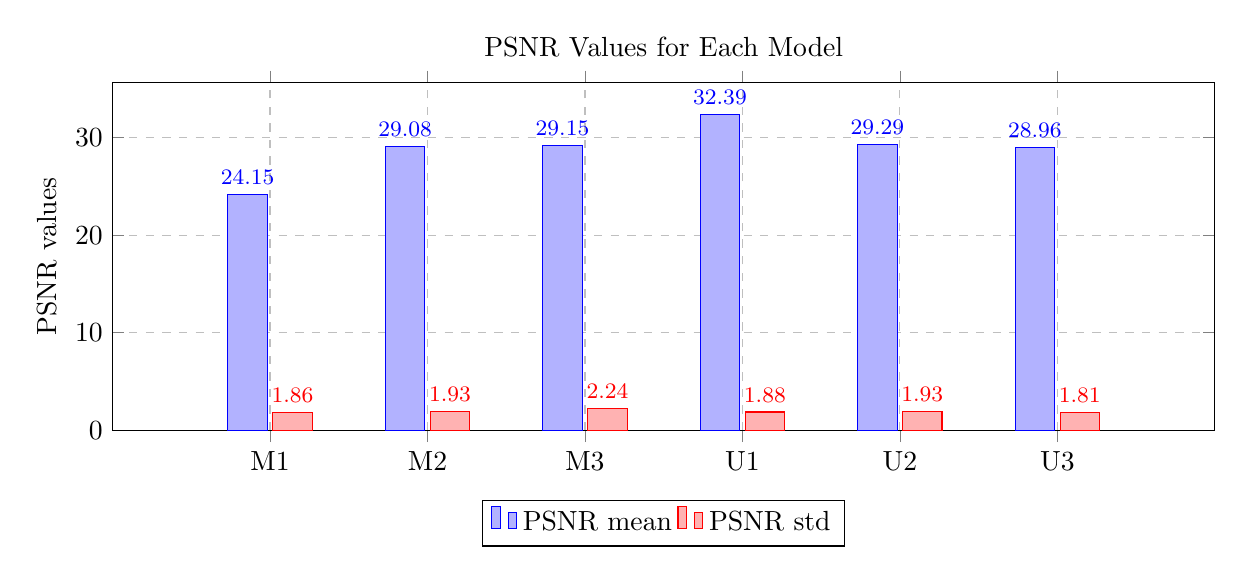
\begin{tikzpicture}
    \begin{axis}
    [ybar, 
    grid = major, major grid style = {dashed},
    ymin = 0,
    ylabel = {PSNR values},
    title = {PSNR Values for Each Model},
    bar width = .5cm,
    width = 40cm,
    height = 6cm,
    symbolic x coords={M1, M2, M3, U1, U2, U3},
    x = 2cm,
    xtick = data,
    nodes near coords,
    nodes near coords style = {font = \fontsize{8}{12}\selectfont},
    enlarge x limits = 0.2,
    legend style = {at = {(0.5,-0.2)},anchor = north,legend columns = -1},
    ] 
    \addplot+ coordinates {(M1, 24.15) (M2, 29.08) (M3, 29.15) (U1, 32.39) (U2, 29.29) (U3, 28.96)}; 
    \addplot+ coordinates {(M1, 1.86) (M2, 1.93) (M3, 2.24) (U1, 1.88) (U2, 1.93) (U3, 1.81)}; 
    \legend{PSNR mean, PSNR std};
    \end{axis} 
  \end{tikzpicture}
  \caption{PSNR Values for Each Model}
  \label{fig:PSNR Values for Each Model}
\end{figure}

\begin{figure}[H]
  \centering
  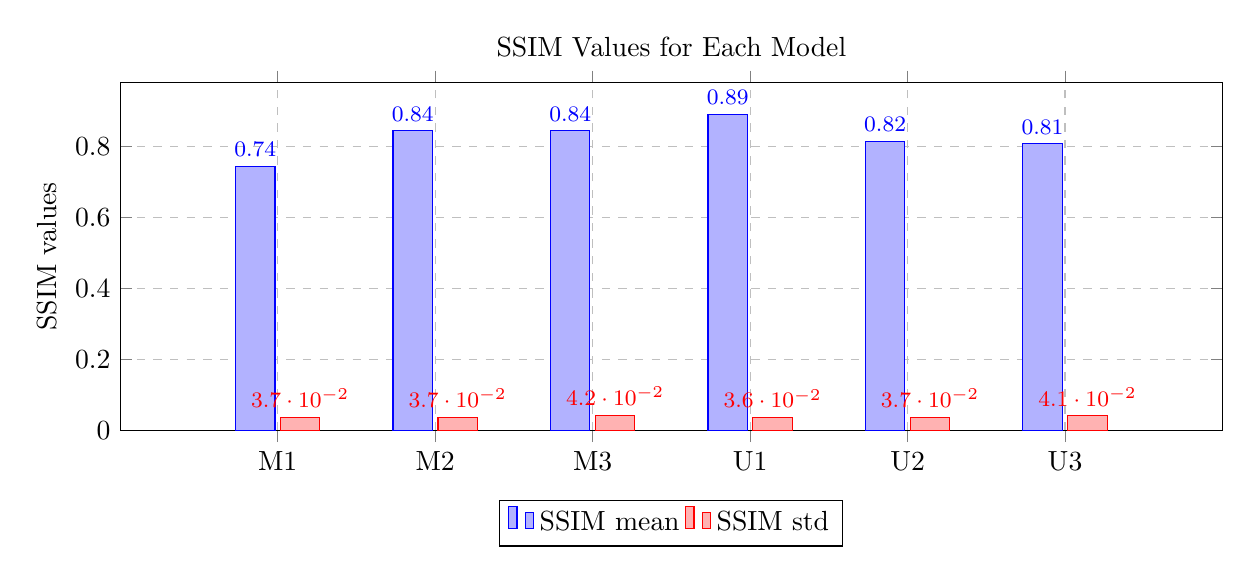
\begin{tikzpicture}
    \begin{axis}
    [ybar, 
    grid = major, major grid style = {dashed},
    ymin = 0,
    ylabel = {SSIM values},
    title = {SSIM Values for Each Model},
    bar width = .5cm,
    width = 40cm,
    height = 6cm,
    symbolic x coords={M1, M2, M3, U1, U2, U3},
    x = 2cm,
    xtick = data,
    nodes near coords,
    nodes near coords style = {font = \fontsize{8}{12}\selectfont},
    enlarge x limits = 0.2,
    legend style = {at = {(0.5,-0.2)},anchor = north,legend columns = -1},
    ] 
    \addplot+ coordinates {(M1, 0.743) (M2, 0.844) (M3, 0.844) (U1, 0.891) (U2, 0.815) (U3, 0.807)}; 
    \addplot+ coordinates {(M1, 0.037) (M2, 0.037) (M3, 0.042) (U1, 0.036) (U2, 0.037) (U3, 0.041)}; 
    \legend{SSIM mean, SSIM std};
    \end{axis} 
  \end{tikzpicture}
  \caption{SSIM Values for Each Model}
  \label{fig:SSIM Values for Each Model}
\end{figure}


%%%%%%%%%%%%%%%%%%%%%%%%%%%%%%%%%%%%%%%%%%%%%%%%%%%%%%%%%%%%


\end{document}